\chapter{Основные теоретические сведения}

\section{Методология ускорения вычислений на основе ПЛИС}

Микропроцессоры и графические процессоры имеют предопределенную архитектуру с фиксированным количеством ядер, набором инструкций, и жесткой архитектурой памяти, и обладают высокими тактовыми частотами и хорошо сбалансированной конвейерной структурой. Графические процессоры масштабируют производительность за счет большого количества ядер и использования параллелизма SIMD/SIMT, что представлено на рисунке \ref{img:scheme}. В отличие от них, программируемые устройства представляют собой полностью настраиваемую архитектуру, которую разработчик может использовать для размещения вычислительных блоков с требуемой функциональностью. В таком случае, высокий уровень производительности достигается за счет создания длинных конвейеров обработки данных, а не за счет увеличения количества вычислительных единиц.

\begin{figure}[H]
	\begin{center}
		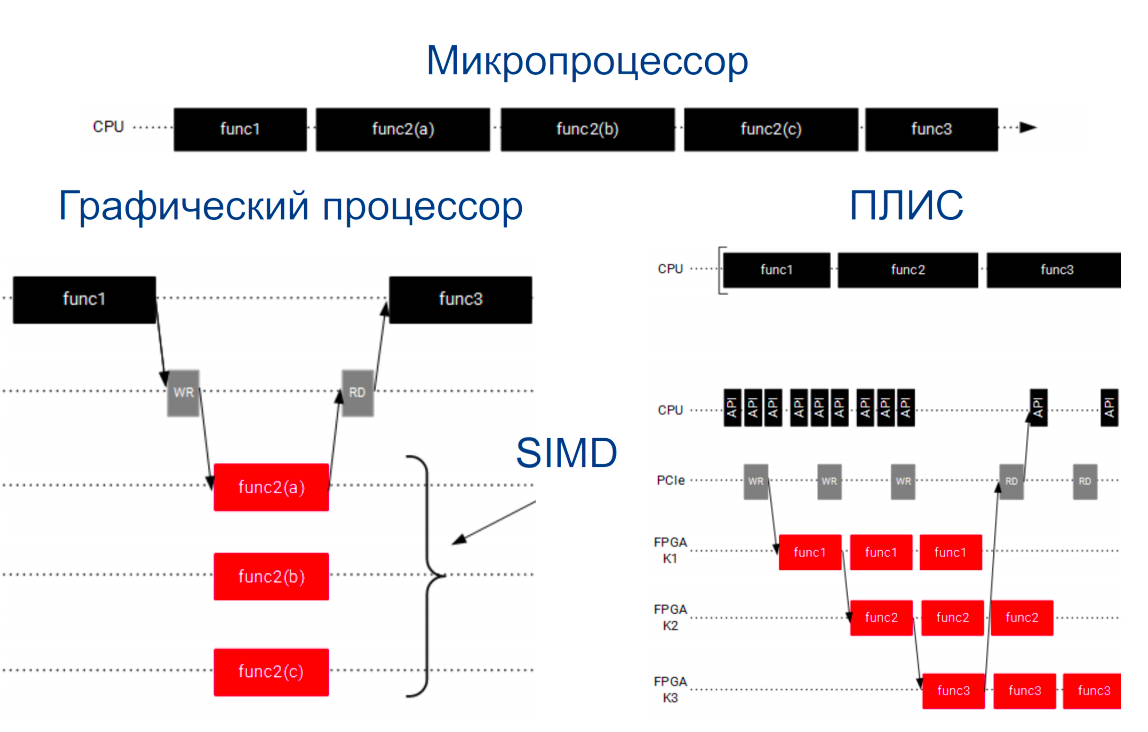
\includegraphics[scale=0.4]{img/scheme.png}
	\end{center}
	\captionsetup{justification=centering}
	\caption{Принципы организации вычислений на различных
платформах}
	\label{img:scheme}
\end{figure}

Методологию создания ускорителей на ПЛИС с применением средств синтеза высокого уровня (High Level Synthesis, HLS) можно представить в виде трех этапов:

\begin{itemize}
	\item создание архитектуры приложения;
	\item разработка ядра аппаратного ускорителя на языках C/C++;
	\item анализ производительности и выявление способов ее повышения.
\end{itemize}

\section{Оптимизация времени обработки и пропускной способности}

Существует несколько подходов к оптимизации.

\subsection{Конвейерная обработка циклов}

Полагая, что одна итерация цикла занимает более одного такта (фаза выборки данных, фаза вычисления, фаза записи результата), может быть организован конвейер выполнения. Для этого необходимо поместить в тело цикла прагму <HLS PIPELINE>.

Без конвейерной обработки каждая последующая итерация цикла начинается через некоторое число тактов. При конвейерной обработке цикл может начинать последующие итерации цикла менее чем за некоторое число тактов, например, в каждом втором такте или в каждом такте.

Стоит отметить, что конвейерная обработка цикла приводит к разворачиванию любых циклов, вложенных внутрь конвейерного цикла. Если внутри цикла существуют зависимости по данным, может оказаться невозможным достичь запуска новой итерации в каждом такте.

\subsection{Разворачивание циклов}

Разворачивание циклов является общепризнанным механизмом снижения времени выполнения циклов. Этот механизм может быть описан самим разработчиком вручную, если он просто повторит вычисления и сократит количество итераций цикла. С помощью прагмы <HLS UNROLL> компилятор v++ позволяет запустить механизм автоматического разворачивания цикла частично или полностью.

\subsection{Потоковая обработка}

Реализация механизма потоковой обработки (\#pragma HLS DATAFLOW) также опирается на представление вычислительных действий в виде многостадийного конвейера. Однако, в то время как директива конвейеризации (\#pragma HLS PIPELINE) используется для реализации конвейера выполнения операций внутри функций или циклов, потоковая обработка данных позволяет сформировать конвейер из более крупных вычислительных блоков: нескольких функций или нескольких последовательных циклических конструкций. Таким образом, директива HLS DATAFLOW позволяет сформировать вычислительный конвейер на уровне задач. Для этих целей компилятор HLS Vitis выполнит анализ зависимостей по данным между задачами и реализует структуру обрабатывающих блоков и FIFO очередей между ними.

\chapter{Функции ядра на основе индивидуального задания}

В листингах \ref{img:no_pragmas}-\ref{img:pipe_unroll} представлены функций ядра: не оптимизированный цикл, конвейерная организация цикла, частично равернутый цикл и конвейерный и частично развернутый цикл.

\begin{figure}[H]
	\begin{center}
		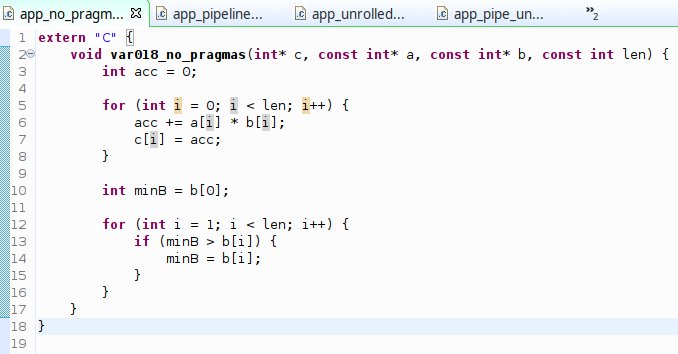
\includegraphics[scale=0.6]{img/no_pragmas.png}
	\end{center}
	\captionsetup{justification=centering}
	\caption{Не оптимизированный цикл на основе индивидуального задания}
	\label{img:no_pragmas}
\end{figure}

\begin{figure}[H]
	\begin{center}
		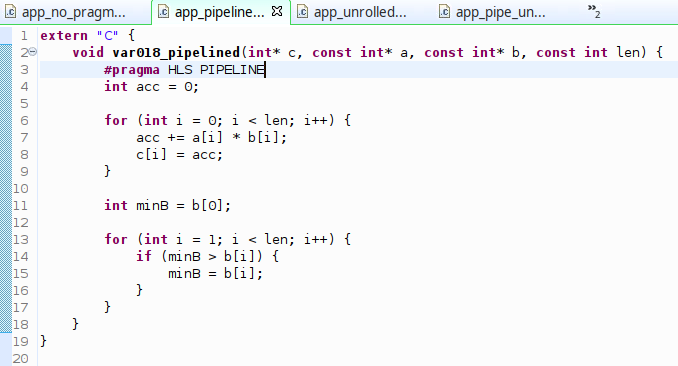
\includegraphics[scale=0.6]{img/pipelined.png}
	\end{center}
	\captionsetup{justification=centering}
	\caption{Конвейерная организация цикла на основе
индивидуального задания}
	\label{img:pipelined}
\end{figure}

\begin{figure}[H]
	\begin{center}
		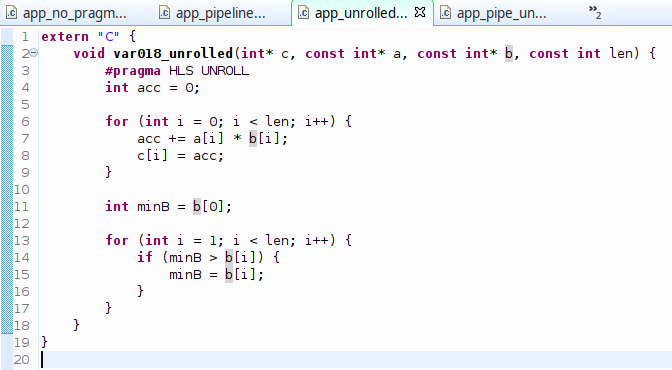
\includegraphics[scale=0.6]{img/unrolled.png}
	\end{center}
	\captionsetup{justification=centering}
	\caption{Частично развернутый цикл на основе индивидуального задания}
	\label{img:unrolled}
\end{figure}

\begin{figure}[H]
	\begin{center}
		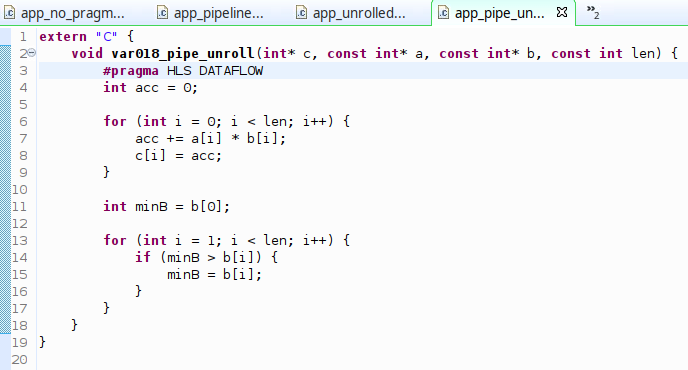
\includegraphics[scale=0.6]{img/pipe_unroll.png}
	\end{center}
	\captionsetup{justification=centering}
	\caption{Конвейерный и частично развернутый цикл
на основе индивидуального задания}
	\label{img:pipe_unroll}
\end{figure}

\chapter{Режим Emulation-SW}

На рисунке \ref{img:sw} показаны результаты рабты приложения в режиме Emulation-SW.

\begin{figure}[H]
	\begin{center}
		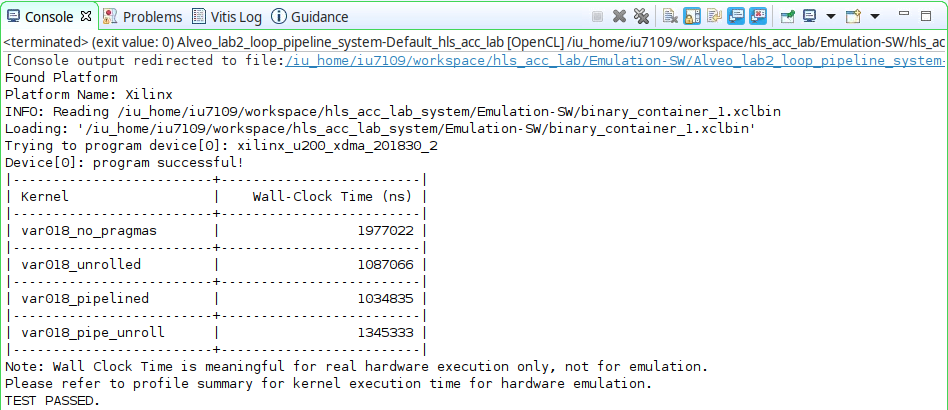
\includegraphics[scale=0.5]{img/sw.png}
	\end{center}
	\captionsetup{justification=centering}
	\caption{Результаты работы приложения в режиме Emulation-SW}
	\label{img:sw}
\end{figure}

\chapter{Режим Emulation-HW}

На рисунке \ref{img:assistant} представлена копия экрана Assistant View для сборки Emulation-HW.

\begin{figure}[H]
	\begin{center}
		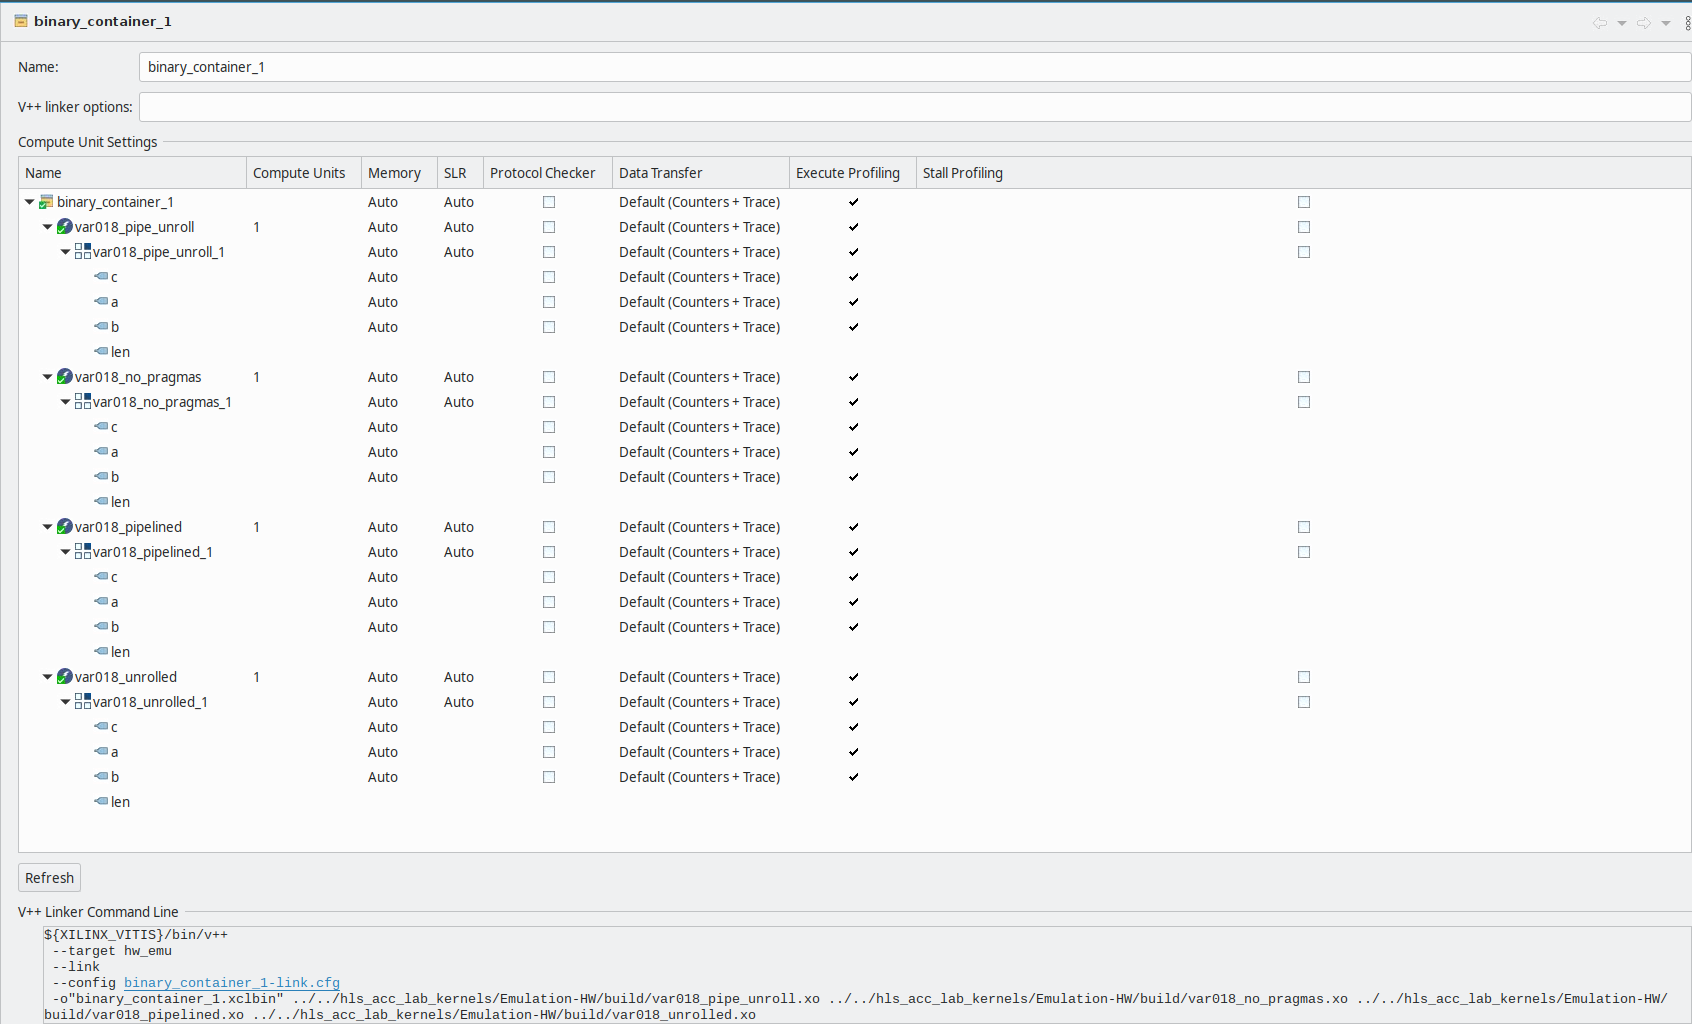
\includegraphics[scale=0.2]{img/assistant.png}
	\end{center}
	\captionsetup{justification=centering}
	\caption{Копия экрана Assistant View для сборки Emulation-HW}
	\label{img:assistant}
\end{figure}

На рисунке \ref{img:hw} показаны результаты работы приложения в режиме Emulation-HW.

\begin{figure}[H]
	\begin{center}
		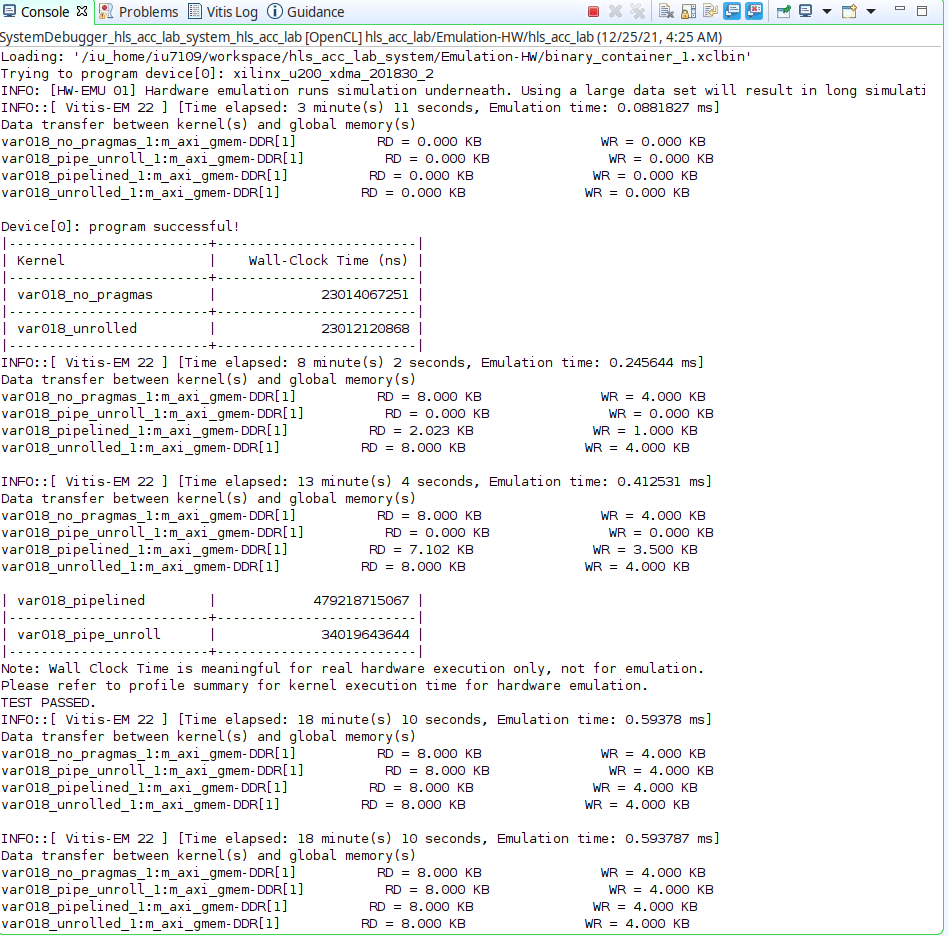
\includegraphics[scale=0.5]{img/hw.png}
	\end{center}
	\captionsetup{justification=centering}
	\caption{Результаты работы приложения в режиме Emulation-HW}
	\label{img:hw}
\end{figure}

Окно внутрисхемного отладчика Vivado для сборки в режиме Emulation-HW представлено на рисунках \ref{img:debugger1}-\ref{img:debugger2}.

\begin{figure}[H]
	\begin{center}
		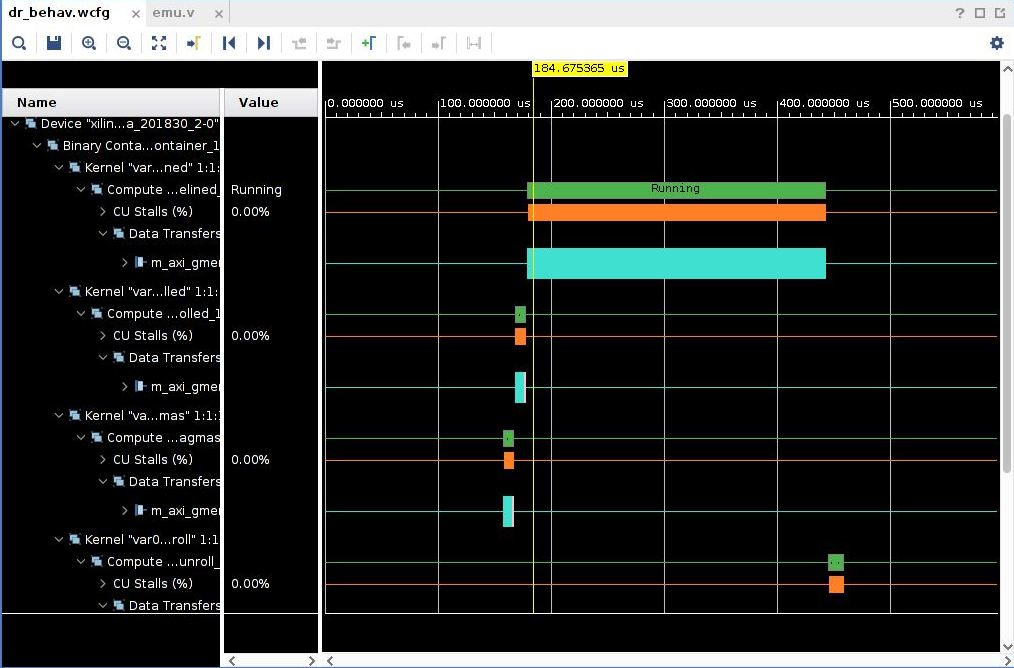
\includegraphics[scale=0.4]{img/debugger1.png}
	\end{center}
	\captionsetup{justification=centering}
	\caption{Окно внутрисхемного отладчика Vivado для сборки в
режиме Emulation-HW - 1}
	\label{img:debugger1}
\end{figure}

\begin{figure}[H]
	\begin{center}
		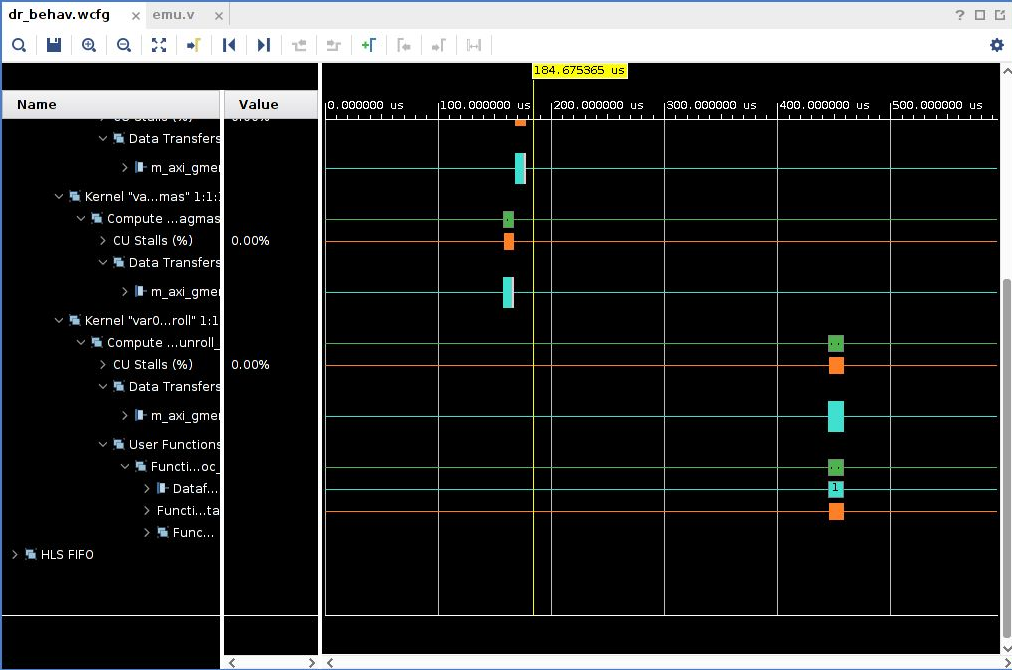
\includegraphics[scale=0.4]{img/debugger2.png}
	\end{center}
	\captionsetup{justification=centering}
	\caption{Окно внутрисхемного отладчика Vivado для сборки в
режиме Emulation-HW - 2}
	\label{img:debugger2}
\end{figure}

\chapter{Режим Hardware}

На рисунке \ref{img:hardware} показаны результаты работы приложения в режиме Hardware.

\begin{figure}[H]
	\begin{center}
		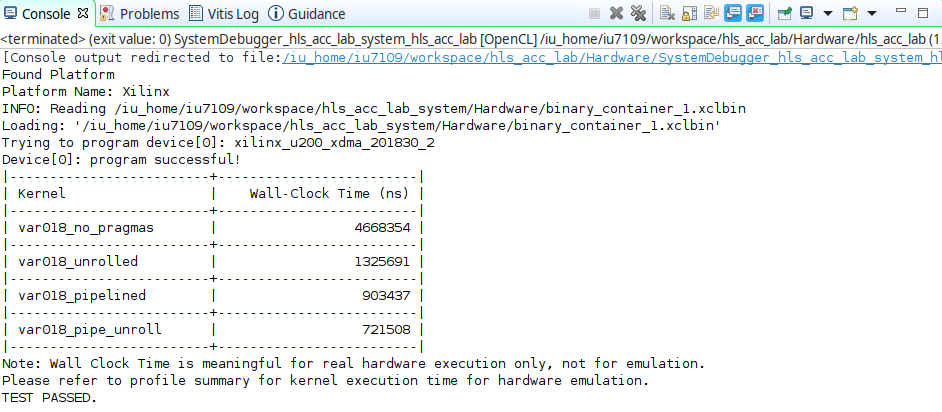
\includegraphics[scale=0.5]{img/hardware.png}
	\end{center}
	\captionsetup{justification=centering}
	\caption{Результаты работы приложения в режиме Hardware}
	\label{img:hardware}
\end{figure}

На рисунках \ref{img:summary}-\ref{img:platform-diagram} представлены копии экранов для вкладок «Summary», «System Diagram», «Platform Diagram».

\begin{figure}[H]
	\begin{center}
		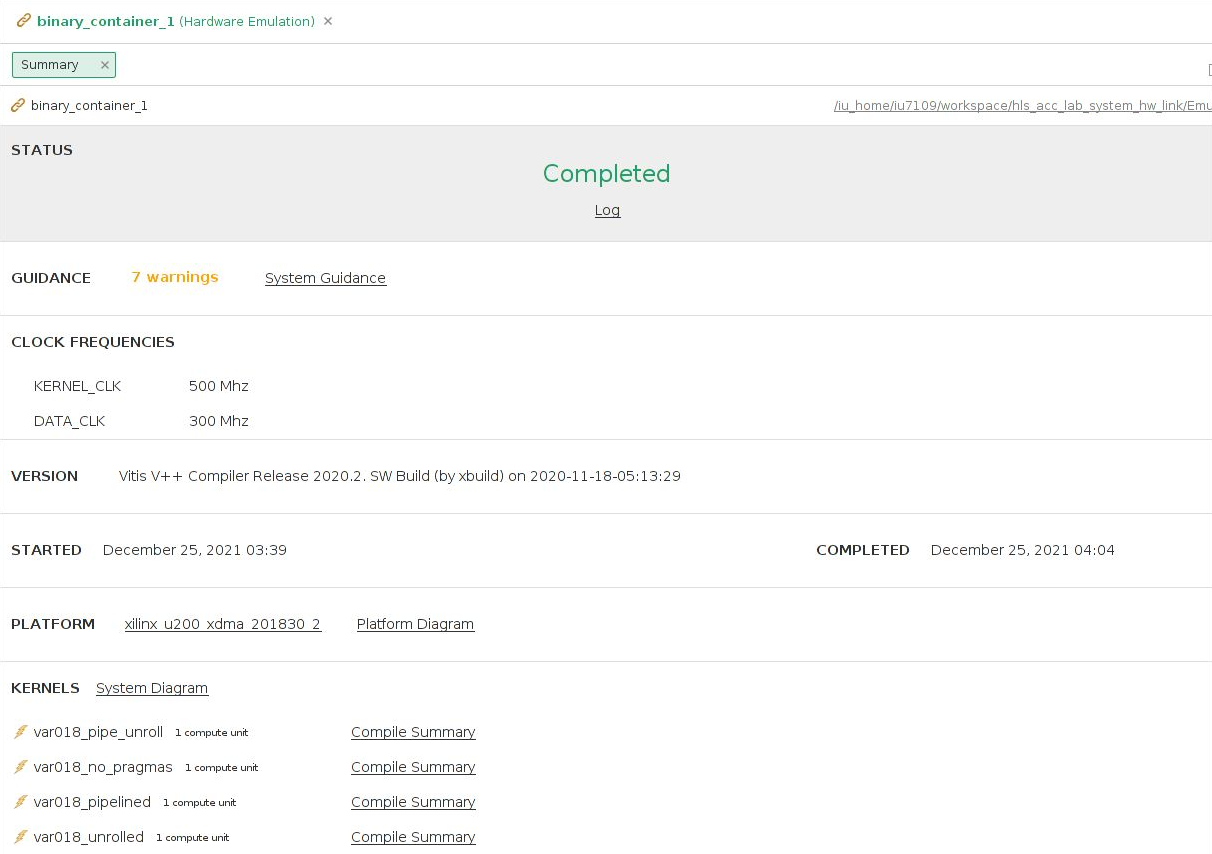
\includegraphics[scale=0.4]{img/summary.png}
	\end{center}
	\captionsetup{justification=centering}
	\caption{Копия экрана вкладки «Summary»}
	\label{img:summary}
\end{figure}

\begin{figure}[H]
	\begin{center}
		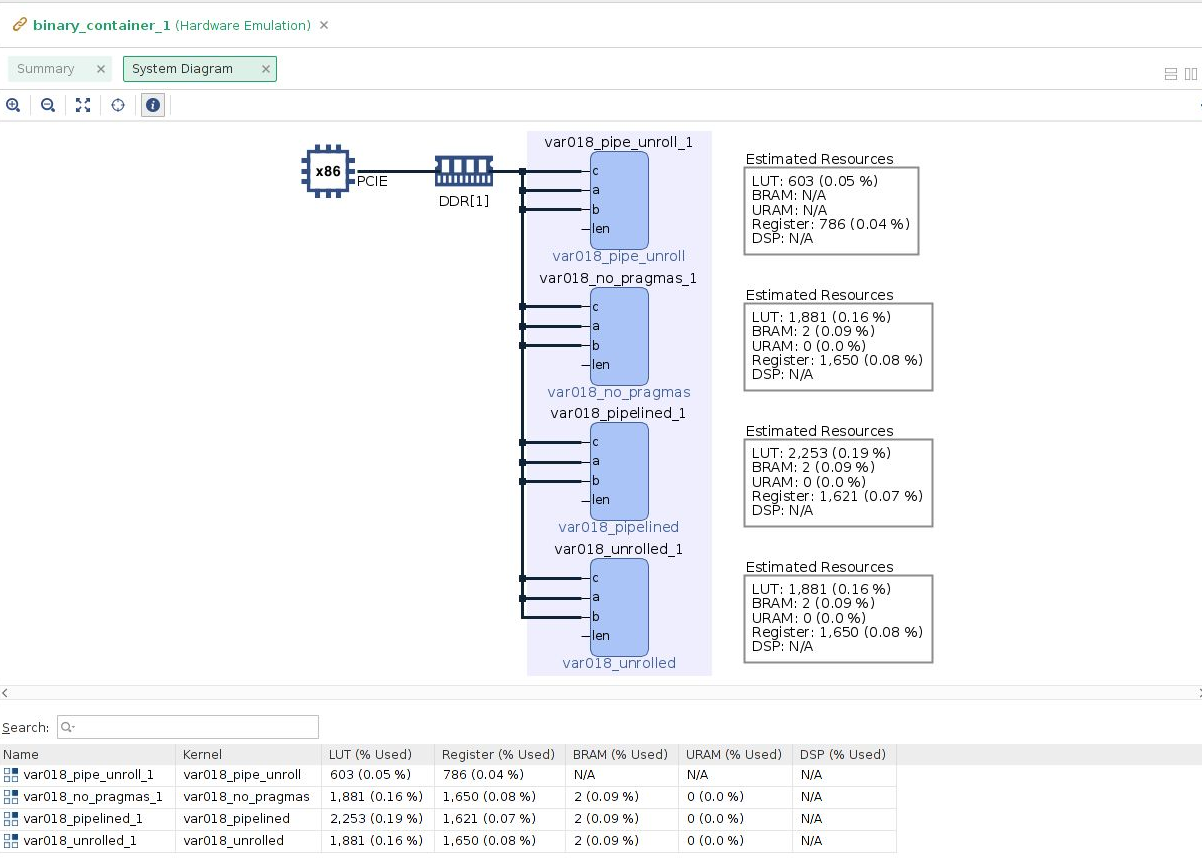
\includegraphics[scale=0.4]{img/system_diagram.png}
	\end{center}
	\captionsetup{justification=centering}
	\caption{Копия экрана вкладки «System Diagram»}
	\label{img:system-diagram}
\end{figure}

\begin{figure}[H]
	\begin{center}
		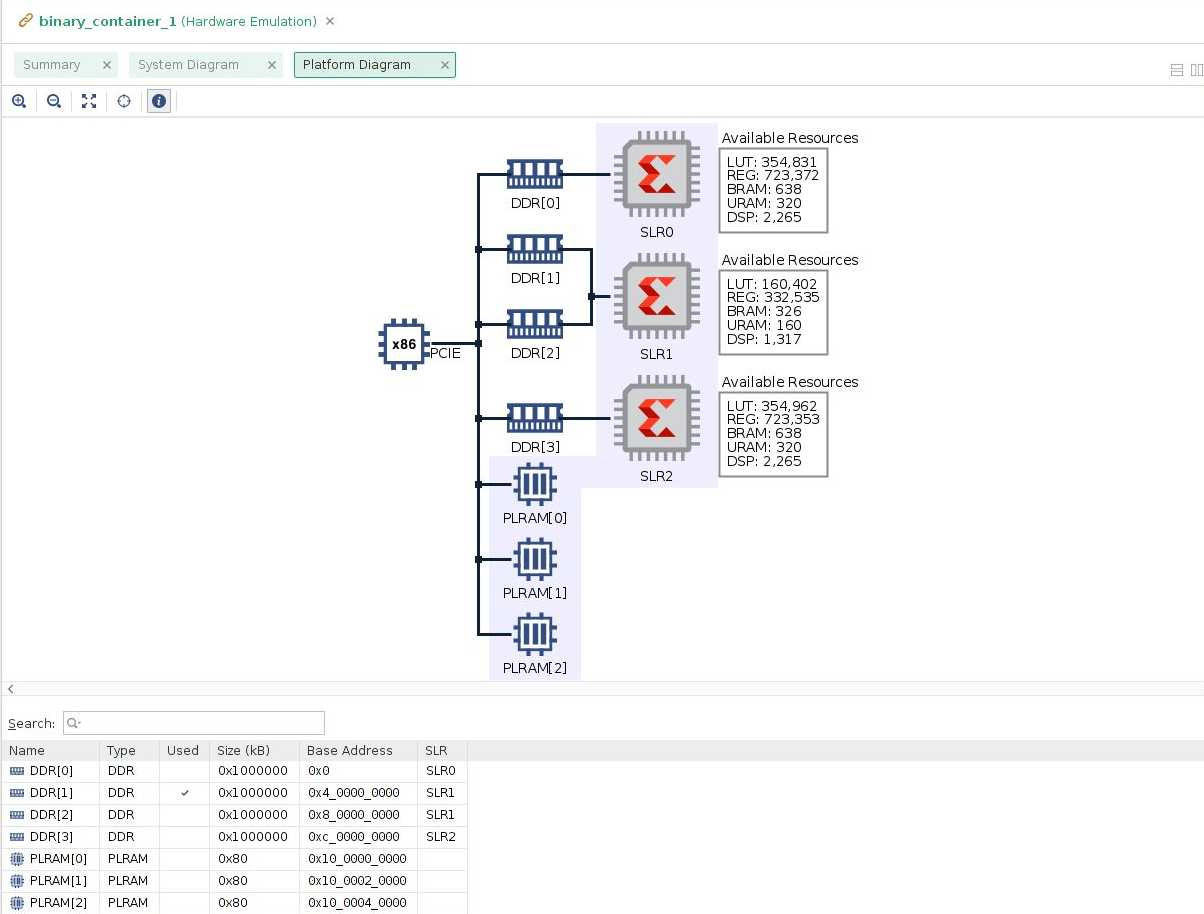
\includegraphics[scale=0.4]{img/platform_diagram.png}
	\end{center}
	\captionsetup{justification=centering}
	\caption{Копия экрана вкладки «Platform Diagram»}
	\label{img:platform-diagram}
\end{figure}

На рисунках \ref{img:hls1}-\ref{img:hls4} показаны копии экранов вкладок «HLS Synthesis» для каждого ядра сборки Hardware.

\begin{figure}[H]
	\begin{center}
		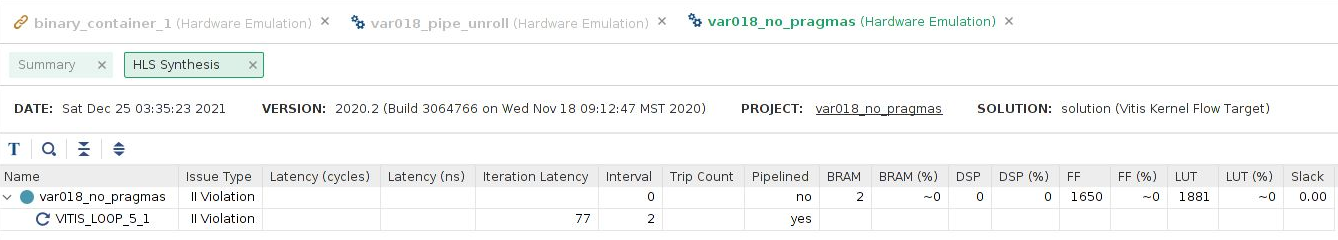
\includegraphics[scale=0.3]{img/hls1.png}
	\end{center}
	\captionsetup{justification=centering}
	\caption{Копия экрана вкладки «HLS Synthesis» для не оптимизированного цикла}
	\label{img:hls1}
\end{figure}

\begin{figure}[H]
	\begin{center}
		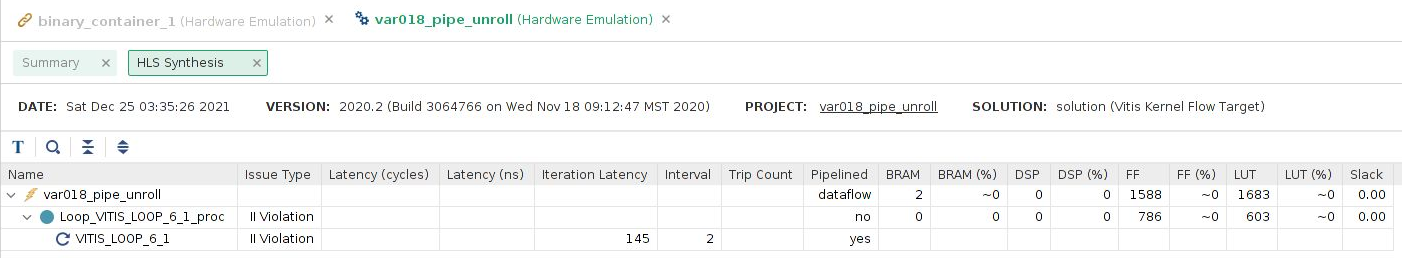
\includegraphics[scale=0.3]{img/hls2.png}
	\end{center}
	\captionsetup{justification=centering}
	\caption{Копия экрана вкладки «HLS Synthesis» для конвейерного и частично развернутого цикла}
	\label{img:hls2}
\end{figure}

\begin{figure}[H]
	\begin{center}
		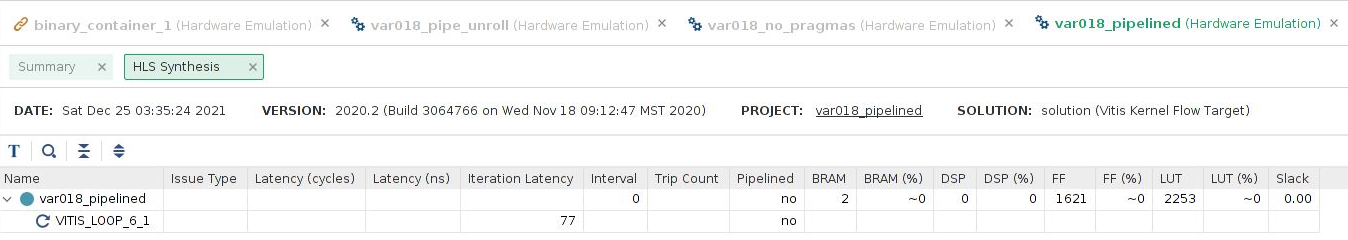
\includegraphics[scale=0.3]{img/hls3.png}
	\end{center}
	\captionsetup{justification=centering}
	\caption{Копия экрана вкладки «HLS Synthesis» для конвейерной организации цикла}
	\label{img:hls3}
\end{figure}

\begin{figure}[H]
	\begin{center}
		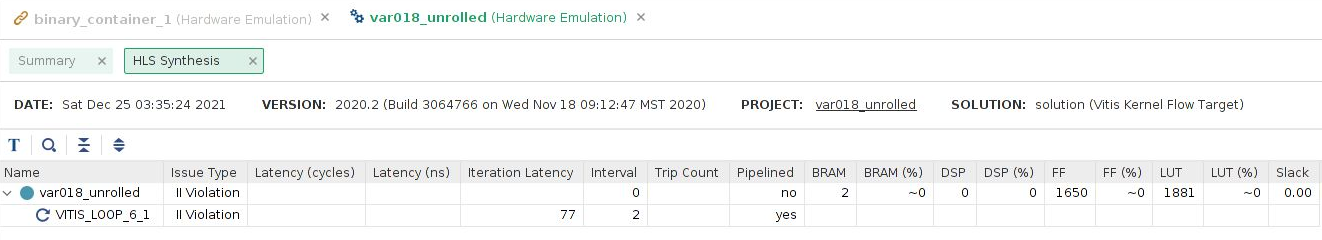
\includegraphics[scale=0.3]{img/hls4.png}
	\end{center}
	\captionsetup{justification=centering}
	\caption{Копия экрана вкладки «HLS Synthesis» для частично развернутого цикла}
	\label{img:hls4}
\end{figure}

\section{Обоснование результатов тестов и выводы}

Из результатов работы приложения в режиме Hardware, показанных на риснуке \ref{img:hardware}, можно сделать вывод о том, что наибольшее время выполнения у не оптимизированного цикла. Наименьшее время выполнения было достигнуто у конвейерного и частично развернутого цикла, так как механизм опирается на представление вычислительных действий в виде многостадийного конвейера.

\chapter{Контрольные вопросы}

\textbf{1. Назовите преимущества и недостатки аппаратных ускорителей на ПЛИС по сравнению с CPU и графическими ускорителями?}

Преимущества аппаратных ускорителей на ПЛИС:
\begin{itemize}
	\item низкая стоимость в сравнении с аппаратными ускорителями;
	\item большая частота эмуляции;
	\item компактность.
\end{itemize}

Недостатки аппаратных ускорителей на ПЛИС:
\begin{itemize}
	\item необходимость перекомпиляции проекта и переконфигурации ПЛИС при любом исправлении содержимого проекта;
	\item наличие специализированного программного обеспечения для разделения модели микросхемы на части для загрузки в отдельные ПЛИС.
\end{itemize}

\textbf{2. Назовите основные способы оптимизации циклических конструкций ЯВУ, реализуемых в виде аппаратных ускорителей?}

Способы оптимизаций циклов:

\begin{itemize}
	\item конвейерная обработка циклов;
	\item разворачивание циклов;
	\item потоковая обработка.
\end{itemize}

\textbf{3. Назовите этапы работы программной части ускорителя в хост-системе?}

Этапы работы программной части ускорителя в хост-системе:
\begin{itemize}
	\item инициализация среды OpenCL;
	\item приложение создает три буфера, необходимых для обмена данными с ядром: два буфера для передачи исходных данных и один для вывода результата;
	\item запуск задачи на исполнение;
	\item после завершения работы всех команд выходной буфер 
содержит результаты работы ядра.
\end{itemize}

\textbf{4. В чем заключается процесс отладки для вариантов сборки Emulation-SW, Emulation-HW и Hardware?}

Для сборки Emulation-SW код ядра компилируется
для работы на ЦПУ хост-системы. Этот вариант сборки служит для
верификации совместного исполнения кода хост-системы и кода ядра, для выявления синтаксических ошибок, выполнения отладки на уровне исходного кода ядра, проверки поведения системы.

Для сборки Emulation-HW код ядра компилируется в
аппаратную модель (RTL), которая запускается в специальном симуляторе на ЦПУ. Этот вариант сборки и запуска занимает больше времени, но обеспечивает подробное и точное представление активности ядра. Данный вариант сборки полезен для тестирования функциональности ускорителя и получения начальных оценок производительности.

Для сборки Hardware код ядра компилируется в аппаратную модель (RTL), а затем реализуется на FPGA. В результате формируется двоичный файл xclbin, который будет работать на реальной FPGA.

\textbf{5. Какие инструменты и средства анализа результатов синтеза возможно использовать в Vitis HLS для оптимизации ускорителей?}

Компилятор Xilinx Vitis v++ позволяет генерировать из описаний на языке C/C++ синтезируемые низкоуровневые RTL проекты, которые затем отображаются на структуру ПЛИС.